In the previous chapter, the required measurement size to obtain an uncertainty of less than \SI{5}{\percent} on the coincidence fraction $f$ was investigated. $f$ is directly accessible from a \gls{BTCCD} analysis. As discussed in Section~\ref{Section:CorrectionForChanceCoincidences}, $f$ systematically overestimates the binding fraction due to the occurrence of chance coincidence events. In the same section, an existing approach to correct for chance coincidences was presented. For the red channel, the corrected coincidence fraction is given by
\begin{equation} \label{Equation:CorrectedCoincidenceFractionRed2}
f_{RB}^{cor}(n_{br}) = \frac{f_{RB}(n_{br}) - f_{RB, 0}^{chance}(n_{br})}{1 - f_{RB, 0}^{chance}(n_{br})},
\end{equation}
where
\begin{equation} \label{Equation:ChanceCoincidenceFractionRed2}
f_{RB, 0}^{chance}(n_{br}) = 1 - \exp\left\{-\left\langle N_B \right\rangle (0) \cdot \left(\frac{\left\langle \tau_d^R\right\rangle (n_{br})}{\left\langle \tau_d^B \right\rangle (0)} + 1\right)\right\}.
\end{equation}
The chance coincidence correction depends on the initial number of blue molecules $\left\langle N_B \right\rangle (0)$ and the dwell time ratio $\left\langle \tau_d^R\right\rangle (n_{br})/ \left\langle \tau_d^B \right\rangle (0)$. For the blue channel, the correction has a similar form and depends on $\left\langle N_R \right\rangle (0)$ and $\left\langle \tau_d^B\right\rangle (n_{br})/ \left\langle \tau_d^R \right\rangle (0)$. In the following, those two parameters are simply called molecule number and dwell time ratio.\\

In the first part of this chapter, see Section~\ref{Section:ApplicationLimits}, it is investigated, for which molecule numbers and dwell time ratios the chance coincidence correction is applicable. Based on experimental data, a method is proposed that allows choosing a suitable molecule number for the measurement of a given sample. Then, in Section~\ref{Section:ApplicatinLimitsValidation}, a trial experiment validates the proposed method.

\section{Application Limits of Chance Coincidence Correction} \label{Section:ApplicationLimits}

\subsection{Measurement} \label{Section:Measurement_Ribosomes_DNA}

To investigate the application limits of the existing chance coincidence correction, two measurement sets were recorded. Table~\ref{Table:Measurement_DNA_Alexa488} contains information on measurement time, burst threshold, background, and starting parameters on seven measurement rows with a mixture of red-labeled \gls{dsDNA} and free Alexa 488. Alexa 488 is a dye that emits blue fluorescence light. It is further referred to as free blue dye. Using \gls{FCS}, the measurement rows were performed with a sample concentration ranged between \SI{20}{\pico\mole\per\liter} and \SI{600}{\pico\mole\per\liter}. The second measurement set was conducted with a mixture of red-labeled ribosomes and free blue dye. Information on measurement time, burst threshold, background, and starting parameters for the six measurement rows can be found in Table~\ref{Table:Measurement_Ribosomes_Alexa488}. Here, the sample concentration lied between \SI{40}{\pico\mole\per\liter} to \SI{1400}{\pico\mole\per\liter}. 

For all measurement rows, using \gls{FCS}, it was determined that the mixture ratio was almost $1:1$.

\vfill
\begin{table}[h!]
	\centering
	\begin{tabular}{c|c|c|c|c|c} 
		ch. & $T$ [\si{\min}] & $\left\langle IPL^{bg} \right\rangle$ [\si{\micro\second}] & $\left\langle N \right\rangle$ [$10^{-3}$] & $\left\langle \tau_d \right\rangle$ [\si{\micro\second}] & $\left\langle MB \right\rangle$ [\si{\kilo\hertz}] \\
		\hline
		red & \multirow{2}{*}{\num{60}} & \num{1585} & \num{15.853 +- 0.086} & \num{776.4 +- 3.1} & \num{47.7 +- 4.0}\\
		blue & & \num{1413} & \num{3.111 +- 0.019} & \num{271.4 +- 1.0} & \num{52.6 +- 5.4} \\
		\hline
		red & \multirow{2}{*}{\num{33}} & \num{282} & \num{78.15 +- 0.29} & \num{878.8 +- 2.3} & \num{44.1 +- 3.2}\\
		blue &  & \num{562} & \num{16.102+- 0.064} & \num{302.22 +- 0.73} & \num{49.7 +- 2.6} \\
		\hline
		red & \multirow{2}{*}{\num{20}} & \num{251} & \num{79.28 +- 0.38} & \num{877.9 +- 3.0} & \num{43.8 +- 1.7}\\
		blue &  & \num{562} & \num{16.167 +- 0.082} & \num{303.54 +- 0.94} & \num{49.1 +- 3.6} \\
		\hline
		red & \multirow{2}{*}{\num{60}} & \num{794} & \num{103.76 +- 0.12} & \num{834.4 +- 2.4} & \num{45.8 +- 1.3}\\
		blue & & \num{355} & \num{23.903 +- 0.060} & \num{321.67 +- 0.49} & \num{47.0 +- 1.8} \\
		\hline
		red & \multirow{2}{*}{\num{20}} & \num{89} & \num{126.312 +- 0.051} & \num{924.1 +- 2.6} & \num{41.5 +- 1.3}\\
		blue &  & \num{251} & \num{46.89 +- 0.16} & \num{360.43 +- 0.72} & \num{42.8 +- 2.2} \\
		\hline
		red & \multirow{2}{*}{\num{18}} & \num{89} & \num{472.2 +- 1.7} & \num{1190.2 +- 2.7} & \num{36.61 +- 0.70}\\
		blue &  & \num{141} & \num{104.04 +- 0.28} & \num{424.87 +- 0.69} & \num{39.6 +- 2.9} \\
		\hline
		red & \multirow{2}{*}{\num{20}} & \num{89} & \num{556.6 +- 2.0} & \num{1259.1 +- 2.7} & \num{36.3 +- 1.3}\\
		blue & & \num{141} & \num{107.99 +- 0.27} & \num{429.64 +- 0.65} & \num{39.4 +- 1.2} \\
		\hline
	\end{tabular}
	\caption[Measurement time, background, and starting parameters for mixture of red-labeled \gls{dsDNA} and free blue dye]{Measurement time, background, and starting parameters for measurements with a mixture of red-labeled \gls{dsDNA} and free blue dye. For all measurements, the burst thresholds were set to $IPL^{tre}_R = \SI{75}{\micro\second}$ and $IPL^{tre}_R = \SI{80}{\micro\second}$. The measurement rows are ordered with increasing sample concentration.}
	\label{Table:Measurement_DNA_Alexa488}
\end{table}
\vfill

\vfill
\begin{table}[h!]
	\centering
	\begin{tabular}{c|c|c|c|c|c|c} 
		ch. & $T$ [\si{\min}] & $IPL^{thr}$ [\si{\micro\second}] & $\left\langle IPL^{bg} \right\rangle$ [\si{\micro\second}] & $\left\langle N \right\rangle$ [$10^{-3}$] & $\left\langle \tau_d \right\rangle$ [\si{\micro\second}] & $\left\langle MB \right\rangle$ [\si{\kilo\hertz}] \\
		\hline
		red & \multirow{2}{*}{\num{60}} & \num{280} & \num{1413} & \num{29.89 +- 0.15} & \num{1193.3 +- 4.2} & \num{24.3 +- 4.6}\\
		blue &  & \num{100} & \num{1259} & \num{4.012 +- 0.024} & \num{326.1 +- 1.2} & \num{46.1 +- 3.8} \\
		\hline
		red & \multirow{2}{*}{\num{53}} & \num{280} & \num{1413} & \num{30.33 +- 0.15} & \num{1171.5 +- 4.0} & \num{23.9 +- 4.7}\\
		blue &  & \num{100} & \num{1413} & \num{3.063 +- 0.022} & \num{324.7 +- 1.5} & \num{45.4 +- 7.7} \\
		\hline
		red & \multirow{2}{*}{\num{20}} & \num{150} & \num{178} & \num{214.23 +- 0.76} & \num{1119.0 +- 2.6} & \num{24.1 +- 2.3}\\
		blue &  & \num{80} & \num{447} & \num{13.643 +- 0.076} & \num{318.2 +- 1.1} & \num{45.2 +- 3.2} \\
		\hline
		red & \multirow{2}{*}{\num{20}} & \num{85} & \num{89} & \num{382.2 +- 1.0} & \num{820.4 +- 1.3} & \num{33.2 +- 1.2}\\
		blue &  & \num{70} & \num{282} & \num{29.54 +- 0.11} & \num{306.36 +- 0.69} & \num{48.0 +- 8.5} \\
		\hline
		red & \multirow{2}{*}{\num{20}} & \num{85} & \num{89} & \num{638.0 +- 1.8} & \num{1050.0 +- 1.6} & \num{31.44 +- 0.92}\\
		blue &  & \num{70} & \num{224} & \num{43.04 +- 0.14} & \num{325.26 +- 0.64} & \num{45.4 +- 1.8} \\
		\hline
		red & \multirow{2}{*}{\num{20}} & \num{60} & \num{89} & \num{1304.9 +- 5.3} & \num{1313.9 +- 2.0} & \num{42.33 +- 0.83}\\
		blue &  & \num{60} & \num{112} & \num{90.71 +- 0.21} & \num{325.18 +- 0.46} & \num{47.5 +- 1.2} \\
	\end{tabular}
	\caption[Measurement time, burst thresholds, background, and starting parameters for mixture of red-labeled ribosomes and free blue dye]{Measurement time, burst thresholds, background, and starting parameters for measurements with a mixture of red-labeled ribosomes and free blue dye. The measurement rows are ordered with increasing sample concentration.}
	\label{Table:Measurement_Ribosomes_Alexa488}
\end{table}
\vfill

\subsection{Results}

As explained above, the coincidence fraction $f$ is directly obtained from the \gls{BTCCD} analysis. For the red channel, $f_{RB}$ is illustrated in Figures~\ref{fig:CoincidenceFraction_DNA_Red} and \ref{fig:CoincidenceFraction_Ribosomes_Red}. The coincidence fraction is depicted for a small, intermediate, and high molecule number. Theoretically, a coincidence fraction of \SI{0}{\percent} is expected because the sample solution contains only single-labeled molecules. Thus, the observed coincidence fraction is assumably only caused by chance coincidences. The chance coincidence fraction becomes more pronounced for a larger molecule number and increases with $n_{br}$. The corresponding results for the blue channel are illustrated in Figures~\ref{fig:CoincidenceFraction_DNA_Blue} and \ref{fig:CoincidenceFraction_Ribosomes_Blue}. For the blue channel, the same dependencies are observed.\\

For the conducted measurements, it is not possible to determine an optimal brightness threshold $n_{br,opt}$ since a coincidence fraction of \SI{0}{\percent} is expected. Therefore, the \gls{BTCCD} analysis was applied for values of $n_{br}$ between \num{0} and \num{10} to cover a reasonable range, in which the optimal brightness threshold typically lies. 

Likewise, the optimal number of bursts criterion from the previous chapter cannot be applied because it refers to the uncertainty of the coincidence fraction at the optimal brightness threshold. Hence, although more than \num{10000} initial bursts were recorded for every measurement, the uncertainty on the blue coincidence fraction becomes notably large for high brightness thresholds. Typically, there are fewer molecules in the blue channel than in the red channel, see e.g. Tables~\ref{Table:Measurement_DNA_Alexa488} and \ref{Table:Measurement_Ribosomes_Alexa488}, because the red confocal detection volume is larger than the blue one. Therefore, the uncertainty on the blue coincidence fraction is more significant than on the red one. \\

To correct for the observed chance coincidences, the existing approach is applied. Figures~\ref{fig:CorrectedCoincidenceFraction_DNA_Red} and \ref{fig:CorrectedCoincidenceFraction_Ribosomes_Red} illustrate the corrected coincidence fraction for the red channel. A systematical deviation of the corrected coincidence fraction from the expected value of \SI{0}{\percent} is observed. The deviation increases with the molecule number and with $n_{br}$. The results for the blue channel can be found in Figures~\ref{fig:CorrectedCoincidenceFraction_DNA_Blue} and \ref{fig:CorrectedCoincidenceFraction_Ribosomes_Blue}. For the blue channel, the deviation from the expected coincidence fraction is not as expressed as in the red channel. More pronounced is the huge uncertainty on the corrected coincidence fraction for higher brightness thresholds. It is the result of the propagation of the uncertainty on the uncorrected coincidence fraction, which, as discussed above, reveals considerable uncertainties.

\begin{figure}[h!]
	\centering
	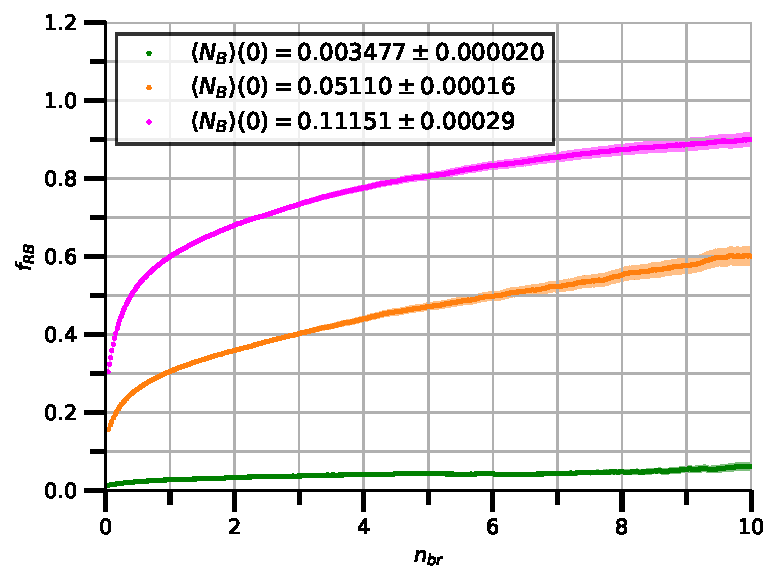
\includegraphics[width=3.9in]{CoincidenceFraction_DNA_Red.pdf}
	\caption[Coincidence fraction of red channel for mixture of red-labeled \gls{dsDNA} and free blue dye]{Coincidence fraction of red channel $f_{RB}$ for the mixture of red-labeled \gls{dsDNA} and free blue dye for a small, intermediate, and high molecule number. The observed coincidence fraction is primarily caused by chance coincidences and increases with $\left\langle N_B \right\rangle (0)$ and $n_{br}$.}
	\label{fig:CoincidenceFraction_DNA_Red}
\end{figure}

\vfill
\begin{figure}[h!]
	\centering
	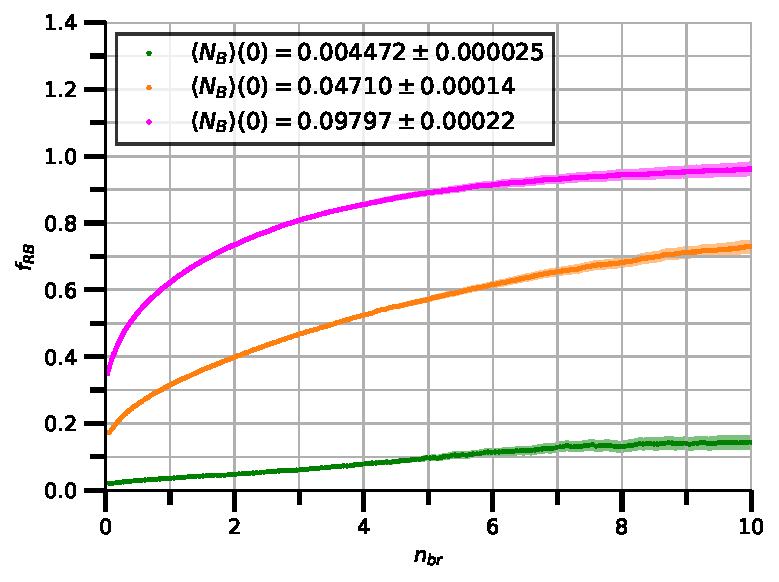
\includegraphics[width=4in]{CoincidenceFraction_Ribosomes_Red.pdf}
	\caption[Coincidence fraction of red channel for mixture of red-labeled ribosomes and free blue dye]{Coincidence fraction of red channel $f_{RB}$ for the mixture of red-labeled ribosomes and free blue dye for a small, intermediate, and high molecule number. The observed coincidence fraction is primarily caused by chance coincidences and increases with $\left\langle N_B \right\rangle (0)$ and $n_{br}$.}
	\label{fig:CoincidenceFraction_Ribosomes_Red}
\end{figure}
\vfill

\vfill
\begin{figure}[h!]
	\centering
	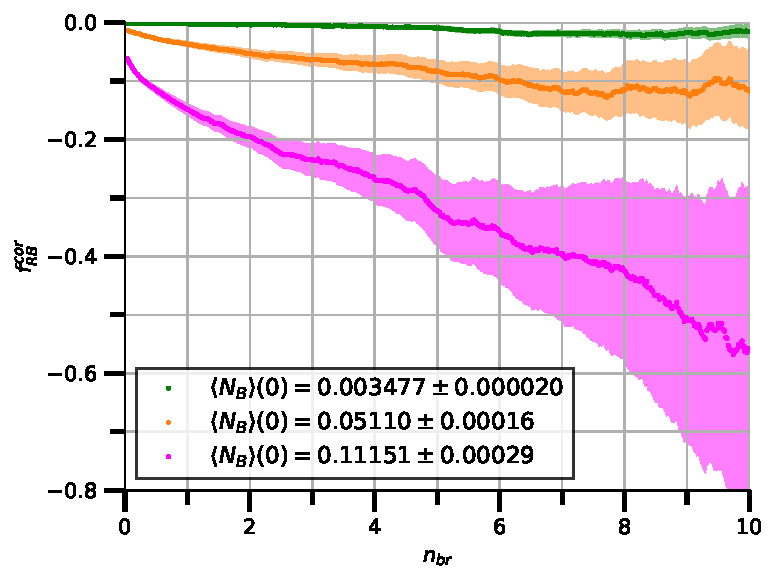
\includegraphics[width=4in]{CorrectedCoincidenceFraction_DNA_Red.pdf}
	\caption[Corrected coincidence fraction of red channel for mixture of red-labeled \gls{dsDNA} and free blue dye]{Corrected coincidence fraction of red channel $f_{RB}^{cor}$ for the mixture of red-labeled \gls{dsDNA} and free blue dye for a low, intermediate, and high molecule number. A deviation of the corrected coincidence fraction from the expected value of \SI{0}{\percent} is observed. The deviation increases with $\left\langle N_B \right\rangle (0)$ and $n_{br}$.}
	\label{fig:CorrectedCoincidenceFraction_DNA_Red}
\end{figure}
\vfill

\begin{figure}[h!]
	\centering
	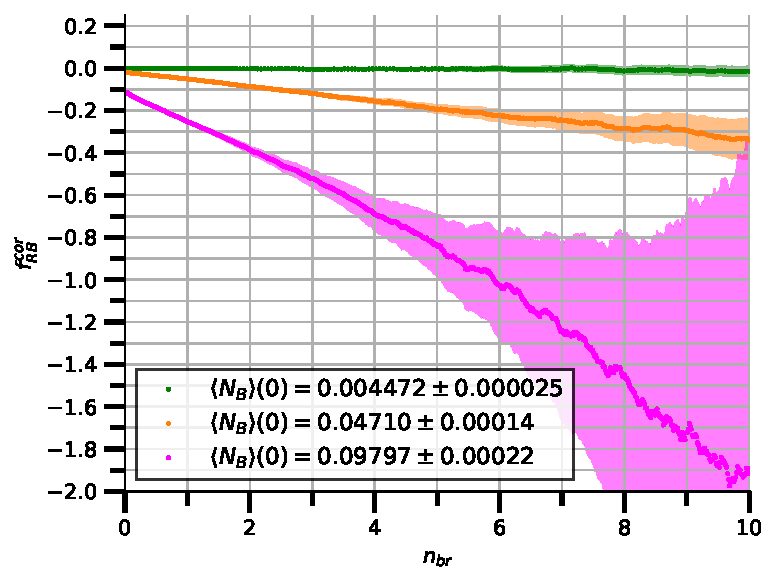
\includegraphics[width=4in]{CorrectedCoincidenceFraction_Ribosomes_Red.pdf}
	\caption[Corrected coincidence fraction of red channel for mixture of red-labeled ribosomes and free blue dye]{Corrected coincidence fraction of red channel $f_{RB}^{cor}$ for the mixture of red-labeled ribosomes and free blue dye for a low, intermediate, and high molecule number. A deviation of the corrected coincidence fraction from the expected value of \SI{0}{\percent} is observed. The deviation increases with $\left\langle N_B \right\rangle (0)$ and $n_{br}$.}
	\label{fig:CorrectedCoincidenceFraction_Ribosomes_Red}
\end{figure}

\subsection{Systematic Deviation of Corrected Coincidence Fraction}

For the conducted measurements, the theoretical coincidence fraction of \SI{0}{\percent} is known. Therefore, the observed coincidence fraction is mostly caused by chance coincidences. According to Equation~\eqref{Equation:ChanceCoincidenceFractionRed2}, the chance coincidence fraction increases with the molecule number and the dwell time ratio. In the measurement results, the dependency on the molecule number was directly observed. To understand the dependency on the dwell time ratio, the knowledge from Section~\ref{Section:DwellTime} that the dwell time ratio is a strictly monotonically increasing function of $n_{br}$ can be used. Then, the observed increase of the coincidence fraction with $n_{br}$ can be explained.\\

It remains the question, why the corrected coincidence fraction deviates clearly from the expected value of \SI{0}{\percent}. For this purpose, it is useful to rewrite the expression for the corrected coincidence fraction, see Equation~\eqref{Equation:CorrectedCoincidenceFractionRed2}, as
\begin{equation} \label{Equation:ChanceCoincidenceCorrectionRewritten_Red}
	f_{RB}^{cor} (n_{br}) = \left(f_{RB}(n_{br}) - f_{RB,0}^{chance}(n_{br})\right) \cdot  \exp\left\{\left\langle N_B \right\rangle (0) \cdot \left(\frac{\left\langle \tau_d^R\right\rangle (n_{br})}{\left\langle \tau_d^B \right\rangle (0)} + 1\right)\right\}.
\end{equation}
The first term describes the deviation of the theoretical expression for the chance coincidence fraction $f_{RB,0}^{chance}$ from the measured coincidence fraction $f_{RB}$. For the conducted measurements, the first term should be approximately \SI{0}{\percent} because the observed coincidence fraction was mostly caused by chance coincidences. The second term describes an exponential increase in terms of the molecule number and the dwell time ratio. It is required to rescale the corrected coincidence fraction because $f_{RB,0}^{chance}$ is derived under the assumption that no real coincidences are present. However, if molecular complexes occur, the effective molecule number that contribute to chance coincidences decreases. The second term takes this phenomenon into account \cite{Hoefig2020}. For the blue channel, the expression for the corrected coincidence fraction can be rewritten similarly. \\
 
First, the deviation of the first term from \SI{0}{\percent} is analyzed. For the red channel, Figures~\ref{fig:ChanceCoincidenceFraction_DNA_Red} and \ref{fig:ChanceCoincidenceFraction_Ribosomes_Red} illustrate the first term for a small, intermediate, and large molecule number. The deviation from the expected value lies roughly between \SI{0}{\percent} and \SI{5}{\percent} for the \gls{dsDNA} measurement, and between \SI{0}{\percent} and \SI{7}{\percent} for the ribosome measurement. The smallest deviation is obtained for a small molecule number. Nonetheless, the deviation does not depend deterministically on the molecule number nor on $n_{br}$. The deviation for the blue channel is shown in Figures~\ref{fig:ChanceCoincidenceFraction_DNA_Blue} and \ref{fig:ChanceCoincidenceFraction_Ribosomes_Blue}. For the blue channel, the deviation of the first term from the expected value is not as much pronounced as for the red channel. The deviation for small brightness thresholds is of the same order as for the red channel. However, for large $n_{br}$, the deviation becomes huge and takes even values of up to \SI{40}{\percent}. As explained above, only a small number of blue bursts remains for these regions, and explains the deviation.\\

So, the first term shows a slight deviation from the expected value of \SI{0}{\percent}. With this knowledge, formally, the first term can be rewritten as 
\begin{equation}
f_{RB}(n_{br}) - f_{RB,0}^{chance}(n_{br}) = f_{RB}^{true}(n_{br}) - f_{RB,0}^{chance,true}(n_{br}) + \Delta f_{RB}(n_{br}).
\end{equation}
Here, $f_{RB}^{true}$ denotes the true coincidence fraction that would be measured if there were no uncertainty. $f_{RB,0}^{chance,true}$ describes an ideal estimation of the chance coincidence fraction. Both quantities are unknown. The deviation between the true and the actual values is absorbed into $\Delta f_{RB}$. Inserting this formulation into Equation~\eqref{Equation:ChanceCoincidenceCorrectionRewritten_Red}, yields 
\begin{align}
f_{RB}^{cor} (n_{br}) &=\nonumber\\ &\left(f_{RB}^{true}(n_{br}) - f_{RB,0}^{chance,true}(n_{br}) + \Delta f_{RB}(n_{br})\right) \cdot  \exp\left\{\left\langle N_B \right\rangle (0) \cdot \left(\frac{\left\langle \tau_d^R\right\rangle (n_{br})}{\left\langle \tau_d^B \right\rangle (0)} + 1\right)\right\}.
\end{align}
Thus, if the first term deviates slightly by $\Delta f_{RB}$ from its true value, the deviation is exponentially amplified by the second term. The specific amplification depends on the molecule number and on the dwell time ratio. Since the dwell time ratio is a function of $n_{br}$, this explains the increasing deviation observed for the corrected coincidence fraction. For the blue channel, the dwell time ratio takes smaller values than for the red channel because the dwell time of blue dye is shorter than that of \gls{dsDNA}. Hence, the systematic deviation in the blue channel is less pronounced. \\

To sum it up, the observed deviation of the corrected coincidence fraction from the expected value of \SI{0}{\percent} is the combination of a slight deviation of the first term and a systematic exponential amplification of the second term. Nonetheless, the latter term is necessary if the coincidence fraction is not expected to be \SI{0}{\percent}, as discussed above. Therefore, a method is required that determines if the existing chance coincidence correction is applicable for a particular molecule number and the corresponding range of the dwell time ratio.

\vfill
\begin{figure}[h!]
	\centering
	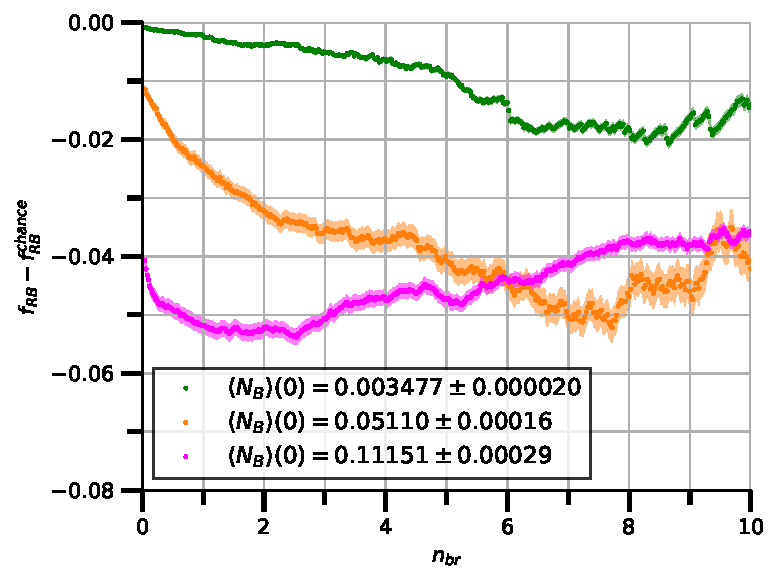
\includegraphics[width=4in]{ChanceCoincidenceFraction_DNA_Red.pdf}
	\caption[First term of corrected coincidence fraction of red channel for mixture of red-labeled \gls{dsDNA} and free blue dye]{First term of corrected coincidence fraction of red channel $f_{RB} - f_{RB,0}^{chance}$ for the mixture of red-labeled \gls{dsDNA} and free blue dye for a small, intermediate, and high molecule number. The expected value of the first term is \SI{0}{\percent}. The deviation from that value lies roughly between \SI{0}{\percent} and \SI{5}{\percent}.}
	\label{fig:ChanceCoincidenceFraction_DNA_Red}
\end{figure}
\vfill

\vfill
\begin{figure}[h!]
	\centering
	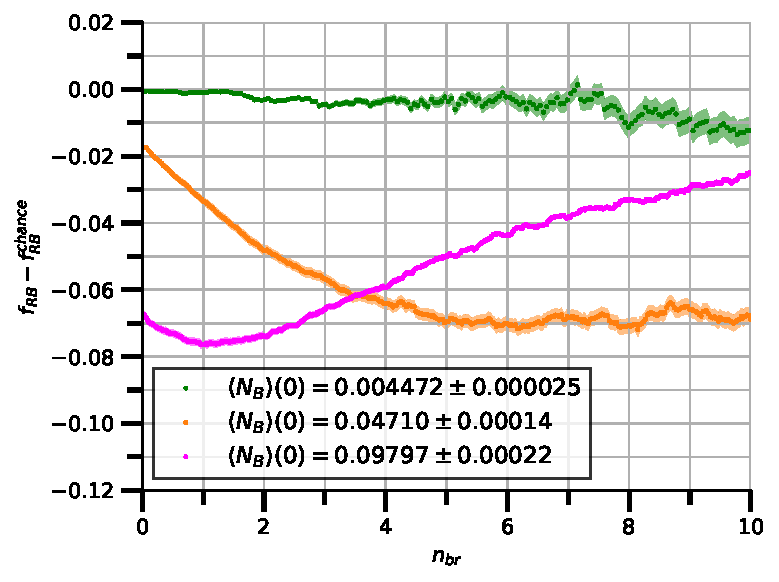
\includegraphics[width=4in]{ChanceCoincidenceFraction_Ribosomes_Red.pdf}
	\caption[First term of corrected coincidence fraction of red channel for mixture of red-labeled ribosomes and free blue dye]{First term of corrected coincidence fraction of red channel $f_{RB} - f_{RB,0}^{chance}$ for the mixture of red-labeled ribosomes and free blue dye for a small, intermediate, and high molecule number. The expected value of the first term is \SI{0}{\percent}. The deviation from that value lies roughly between \SI{0}{\percent} and \SI{7}{\percent}.}
	\label{fig:ChanceCoincidenceFraction_Ribosomes_Red}
\end{figure}
\vfill

\subsection{Application Range of Chance Coincidence Correction}

The application range of the existing chance coincidence correction can be derived from the conducted measurements. For this purpose, two criteria are defined, to decide, whether the chance coincidence correction leads to consistent results. Both the deviation of the corrected coincidence fraction and its statistical uncertainty should not exceed \SI{5}{\percent}. The motivation for the second criterion is that it does not make sense to search for a systematic deviation if the statistical uncertainty is already of the same order. The concrete threshold of \SI{5}{\percent} is based on typical requirements on the accuracy of the binding fraction. \\

Figure~\ref{fig:PossibleRanges_Red} illustrates the application range for the red channel. For every measured molecule number, the range of the dwell time ratio for which the criteria are fulfilled is plotted as a vertical line. Remember, that the dwell time ratio is a strictly monotonically increasing function of $n_{br}$. Hence, the lowest dwell time ratio corresponds to $n_{br} = 0$. There are two possible reasons why the vertical lines end at a particular dwell time ratio. One reason is that the criteria are not anymore fulfilled for larger dwell time ratios. In the figure, this case is marked with a short horizontal line at the highest dwell time ratio. If the criterion holds for the whole range of brightness thresholds from \num{0} to \num{10}, the ending is not specifically marked. A simple dot denotes that the criteria are not fulfilled for the whole range of dwell time ratios. As expected, the application range of the chance coincidence correction in terms of the dwell time ratio decreases for larger molecule numbers. \\

The next step is to interpolate the obtained results for the application range, see Figure~\ref{fig:ReferenceGraph_Red}. The interpolation allows to determine the application range for an arbitrary molecule number. Note that the interpolation serves only for illustration and is not calculated from a theoretical relation. It is solely based on the obtained measurement results.\\

So far, the application range in terms of the dwell time ratio can be determined for every molecule number. The sample concentration roughly specifies the molecule number. In contrast, to obtain knowledge on the range of the dwell time ratio, an accelerated \gls{BTCCD} can be applied. There, the dwell time ratio for $n_{br} = 0$ and for a larger brightness threshold is calculated. Prior to a precise measurement, the optimal brightness threshold $n_{br,opt}$ is unknown. Therefore, it is advised to consider a range of $n_{br}$ in which $n_{br,opt}$ typically lies, and to calculate the dwell time ratio for the high brightness threshold. If the range of dwell time ratios does not lie completely in the application range of the chance coincidence correction, the molecule number needs to be decreased. Otherwise, it is not ensured that the chance coincidence correction is applicable at the optimal brightness threshold. \\

For the blue channel, the raw data for the application range of the chance coincidence correction and the interpolation can be found in Figures~\ref{fig:PossibleRanges_Blue} and \ref{fig:ReferenceGraph_Blue}. The main limit for the blue channel is that the statistical uncertainty on the corrected coincidence fraction exceeds \SI{5}{\percent}. Due to the relative low number of bursts for high brightness thresholds, it becomes considerable large for large dwell time ratios.

\vfill
\begin{figure}[h!]
	\centering
	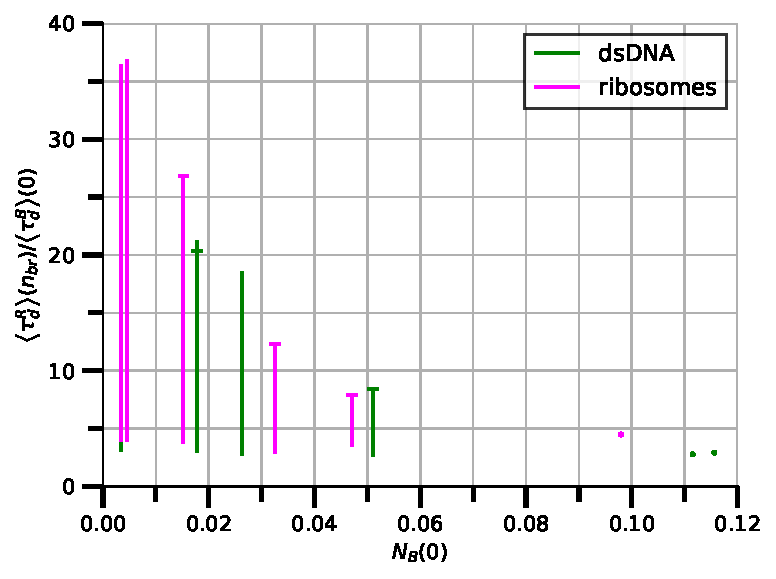
\includegraphics[width=4in]{PossibleRanges_Red.pdf}
	\caption[Application range of chance coincidence correction for red channel for measurements with \gls{dsDNA} and ribosomes]{Application range in terms of dwell time ratio as a function of the molecule number for the red channel. Every vertical line represents one measurement. A short horizontal line at the highest dwell time ratio indicates that the deviation of the corrected coincidence fraction or its statistical uncertainty becomes more than \SI{5}{\percent} for higher dwell time ratios. A simple dot denotes that the chance coincidence correction is unsuitable for the whole measurement.}
	\label{fig:PossibleRanges_Red}
\end{figure}
\vfill

\vfill
\begin{figure}[h!]
	\centering
	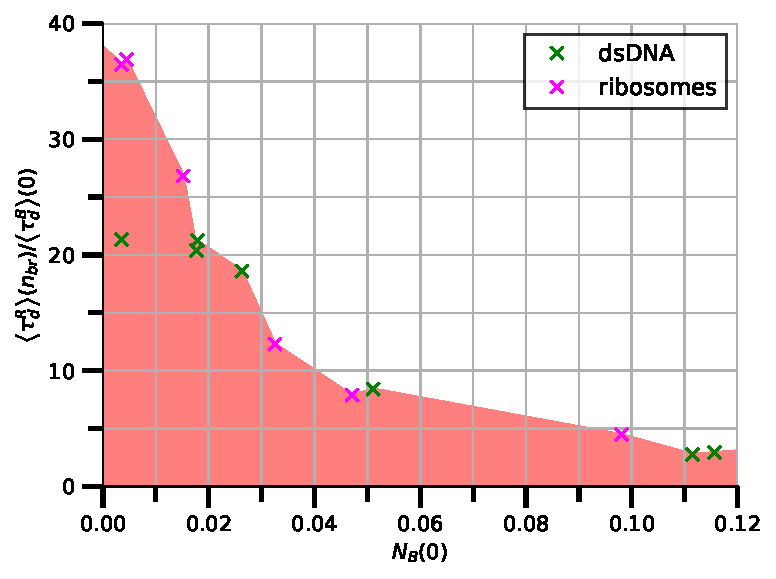
\includegraphics[width=4in]{ReferenceGraph_Red.pdf}
	\caption[Interpolated application range of chance coincidence correction for red channel for measurements with \gls{dsDNA} and ribosomes]{Interpolated application range in terms of dwell time ratio as a function of the molecule number for the red channel. The interpolation serves only for illustration and is not derived from theoretical knowledge. It allows to determine the application range for an arbitrary molecule number.}
	\label{fig:ReferenceGraph_Red}
\end{figure}
\vfill

\clearpage

\section{Validation of Application Limits} \label{Section:ApplicatinLimitsValidation}

\subsection{Measurement} \label{Section:ValdiationMeasurement}

Six measurement rows with a mixture of red-labeled \gls{dsDNA} and dual-labeled \gls{dsDNA} were conducted. Using \gls{FCS}, it was de
termined that the mixture ratio was almost $1:1$. Information on measurement time, burst thresholds, background, and starting parameters can be found in Table~\ref{Table:Measurement_rlDNA_dlDNA}. The sample concentration ranged between \SI{10}{\pico\mole\per\liter} and \SI{400}{\pico\mole\per\liter}.

\begin{table}[h]
	\centering
	\begin{tabular}{c|c|c|c|c|c|c} 
		ch. & $T$ [\si{\min}] & $IPL^{thr}$ [\si{\micro\second}] & $\left\langle IPL^{bg} \right\rangle$ [\si{\micro\second}] & $\left\langle N \right\rangle$ [$10^{-3}$] & $\left\langle \tau_d \right\rangle$ [\si{\micro\second}] & $\left\langle MB \right\rangle$ [\si{\kilo\hertz}] \\
		\hline
		red & \multirow{2}{*}{\num{60}} & \num{120} & \num{1778} & \num{17.95 +- 0.11} & \num{1223.1 +- 5.3} & \num{34.5 +- 1.5}\\
		blue &  & \num{120} & \num{2512} & \num{2.407 +- 0.030} & \num{783.6 +- 6.3} & \num{28.7 +- 3.9} \\
		\hline
		red & \multirow{2}{*}{\num{60}} & \num{120} & \num{1413} & \num{25.78 +- 0.13} & \num{1202.3 +- 4.3} & \num{34.1 +- 1.5}\\
		blue &  & \num{120} & \num{891} & \num{4.507 +- 0.037} & \num{634.3 +- 3.3} & \num{23.6 +- 1.2} \\
		\hline
		red & \multirow{2}{*}{\num{20}} & \num{100} & \num{316} & \num{91.70 +- 0.46} & \num{1137.2 +- 4.0} & \num{35.5 +- 2.0}\\
		blue &  & \num{100} & \num{794} & \num{9.754 +- 0.093} & \num{618.3 +- 3.8} & \num{28.7 +- 2.2} \\
		\hline
		red & \multirow{2}{*}{\num{20}} & \num{100} & \num{200} & \num{122.89 +- 0.56} & \num{1169.4 +- 3.7} & \num{33.5 +- 1.5}\\
		blue &  & \num{100} & \num{708} & \num{12.68 +- 0.11} & \num{622.8 +- 3.3} & \num{27.6 +- 1.1} \\
		\hline
		red & \multirow{2}{*}{\num{20}} & \num{60} & \num{89} & \num{741.2 +- 2.8} & \num{1317.1 +- 2.8} & \num{37.2 +- 1.0}\\
		blue &  & \num{100} & \num{251} & \num{68.34 +- 0.29} & \num{745.4 +- 2.1} & \num{26.86 +- 0.64} \\
		\hline
		red & \multirow{2}{*}{\num{20}} & \num{60} & \num{89} & \num{757.1 +- 2.7} & \num{1142.4 +- 2.3} & \num{41.9 +- 1.7}\\
		blue &  & \num{100} & \num{251} & \num{78.53 +- 0.32} & \num{758.3 +- 2.0} & \num{27.00 +- 0.68} \\
	\end{tabular}
	\caption[Measurement time, burst thresholds, background, and starting parameters for measurements of mixture of red-labeled \gls{dsDNA} and dual-labeled \gls{dsDNA}]{Measurement time, burst thresholds, background, and starting parameters for measurements of a mixture of red-labeled \gls{dsDNA} and dual-labeled \gls{dsDNA}. The measurement rows are ordered with increasing sample concentration.}
	\label{Table:Measurement_rlDNA_dlDNA}
\end{table}

\subsection{Results and Discussion}

To validate the application limits of the chance coincidence correction, first, the optimal brightness threshold for the six measurement rows is determined. Table~\ref{Table:ValidationOpt_Red} gives an overview of the results for the red channel. Besides the optimal brightness threshold, it includes the molecule number, the relevant dwell time ratio, the uncorrected coincidence fraction, and the corrected coincidence fraction. The position of the optimal brightness thresholds in the application range illustration from the previous chapter can be found in Figure~\ref{fig:ReferenceGraphValidation_Red}. The first four measurement rows lie definitively in the application range, while the two measurement rows with the highest concentration are outside it. In general, the measurement results reflect the mixing ratio of $1:1$ as the corrected coincidence fraction is roughly \SI{50}{\percent}. Hence, a reasonable guess for the actual binding fraction is the corrected coincidence fraction for the first measurement. There, the molecule number is small, and it is expected that the chance coincidence correction leads to accurate results. Then, the other measurements can be compared with this reference value. Here, the corrected coincidence fractions spread around the first value, and no systematic trend is observable. \\ 

The optimal brightness threshold is different for every measurement row. This complicates the observation of systematical deviations because the coincidence fractions vary additionally. Hence, another approach is to compare the corrected coincidence fractions for a fixed brightness threshold. Here, the optimal brightness threshold $n_{br} = \num{6.40}$ of the first measurement row is taken as that value. The results are displayed in Table~\ref{Table:Validation_Red}. It can be seen that the two measurement rows with the highest molecule number deviate by \SI{3.9}{\percent} and \SI{5.1}{\percent}, respectively, from the first measurement row. For those measurement rows, a deviation is expected as they lie outside the application range, see Figure~\ref{fig:ReferenceGraphValidation_Red}. \\

\vfill
\begin{table}[h!]
	\centering
	\begin{tabular}{c|c|c|c|c} 
		$n_{br,opt}$ & $\left\langle N_B \right\rangle (0)$ [$10^{-3}$] & $\left\langle \tau_d^R \right\rangle(n_{br,opt})/ \left\langle \tau_d^B  \right\rangle(0)$ & $f_{RB}(n_{br,opt})$ [\si{\percent}] & $f_{RB}^{cor}(n_{br,opt})$ [\si{\percent}] \\
		\hline
		\num{6.40} & \num{2.529 +- 0.030} & \num{7.480 +- 0.016} & \num{50.7 +- 2.3} & \num{49.6 +- 2.3} \\
		\num{5.04} & \num{5.057 +- 0.037} & \num{8.977 +- 0.010} & \num{46.3 +- 1.4} & \num{43.5 +- 1.5} \\
		\num{5.05} & \num{10.538 +- 0.094} & \num{8.987 +- 0.011} & \num{52.8 +- 1.3} & \num{47.6 +- 1.5} \\
		\num{8.37} & \num{13.68 +- 0.11} & \num{12.479 +- 0.011} & \num{61.9 +- 2.2} & \num{54.2 +- 2.7} \\
		\num{9.28} & \num{72.52 +- 0.29} & \num{15.8994 +- 0.0056} & \num{85.2 +- 1.3} & \num{49.7 +- 4.4} \\
		\num{9.63} & \num{83.21 +- 0.32} & \num{14.2016 +- 0.0053} & \num{86.3 +- 1.2} & \num{51.3 +- 4.4} 
	\end{tabular}
	\caption[Corrected coincidence fraction of red channel at optimal brightness threshold for a mixture of red-labeled \gls{dsDNA} and dual-labeled \gls{dsDNA}]{Corrected coincidence fraction $f_{RB}^{cor}$ of red channel at the optimal brightness threshold $n_{br,opt}$ for measurements with a mixture of red-labeled \gls{dsDNA} and dual-labeled \gls{dsDNA}. For every measurement row, the molecule number, the relevant dwell time ratio, and the uncorrected coincidence fraction are stated. The first measurement is taken as a guess for the true binding fraction. The corrected coincidence fractions spread around the first value, and no systematic trend is observable.}
	\label{Table:ValidationOpt_Red}
\end{table}
\vfill

\vfill
\begin{table}[h!]
	\centering
	\begin{tabular}{c|c|c|c} 
		$\left\langle N_B \right\rangle (0)$ [$10^{-3}$] & $\left\langle \tau_d^R \right\rangle(6.40)/ \left\langle \tau_d^B  \right\rangle(0)$ & $f_{RB}(6.40)$ [\si{\percent}] & $f_{RB}^{cor}(6.40)$ [\si{\percent}] \\
		\hline
		\num{2.529 +- 0.030} & \num{7.480 +- 0.016} & \num{50.7 +- 2.3} & \num{49.6 +- 2.3} \\
		\num{5.057 +- 0.037} & \num{10.225 +- 0.011} & \num{48.7 +- 1.9} & \num{45.7 +- 2.0} \\
		\num{10.538 +- 0.094} & \num{10.053 +- 0.012} & \num{55.2 +- 1.7} & \num{49.7 +- 1.9} \\
		\num{13.68 +- 0.11} & \num{10.711 +- 0.012} & \num{59.5 +- 1.6} & \num{52.4 +- 1.9} \\
		\num{72.52 +- 0.29} & \num{12.9324 +- 0.0052} & \num{80.24 +- 0.87} & \num{45.7 +- 2.5} \\
		\num{83.21 +- 0.00032} & \num{11.2796 +- 0.0048} & \num{80.00 +- 0.80} & \num{44.5 +- 2.3} 
	\end{tabular}
	\caption[Corrected coincidence fraction of red channel at $n_{br} = \num{6.40}$ for a mixture of red-labeled \gls{dsDNA} and dual-labeled \gls{dsDNA}]{Corrected coincidence fraction $f_{RB}^{cor}$ of red channel at $n_{br} = \num{6.40}$ for measurements with a mixture of red-labeled \gls{dsDNA} and dual-labeled \gls{dsDNA}. For every measurement row, the molecule number, the relevant dwell time ratio, and the uncorrected coincidence fraction are stated. The first measurement is taken as a guess for the true binding fraction. The last two corrected coincidence fractions corresponding to the highest molecule numbers deviate by \SI{3.9}{\percent} and \SI{5.1}{\percent} from the first one.}
	\label{Table:Validation_Red}
\end{table}
\vfill

\clearpage

\begin{figure}[h!]
	\centering
	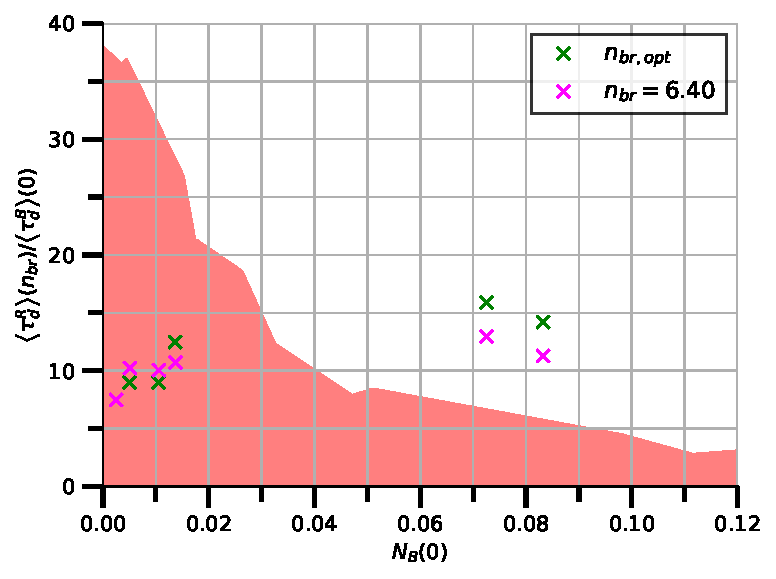
\includegraphics[width=4in]{ReferenceGraphValidation_Red.pdf}
	\caption[Positions of validation measurements in application range illustration for red channel]{Position of the validation experiments for the optimal brightness threshold (see Table~\ref{Table:ValidationOpt_Red}) and for $n_{br} = \num{6.40}$ (see Table~\ref{Table:Validation_Red}) in the illustration of the application range of the chance coincidence fraction for the red channel. The first four measurements lie definitively in the application range, while the two measurements with the highest concentration are outside it.}
	\label{fig:ReferenceGraphValidation_Red}
\end{figure}

The observed deviation from the reference value is still small. This is caused by the relative small dwell time ratios compared to those for the mixtures of ribosomes and free dye in the previous chapter. For the analysis of the application limits, it would be useful to measure samples with different diffusing properties that lead to larger dwell time ratios. Then, a clearer systematic trend would be expected. However, yet, such measurements are not possible due to an existing shortcoming of \gls{BTCCD}. It cannot be applied for samples with significantly different initial dwell times if the binding fraction is larger than \SI{0}{\percent}. \footnote{For the mixtures of ribosomes and free dye in the previous chapter, the dwell times differed significantly. However, since the expected binding fraction was \SI{0}{\percent}, \gls{BTCCD} was applicable.} The reason for this is that, if a complex between the molecule types is formed, it has necessarily a larger dwell time than the faster molecule. Then, the application of a brightness threshold will exclude bursts corresponding to the faster single molecule because they are considered as dim compared to the bursts of the complex. Thus, for large $n_{br}$, the coincidence fraction falsely approaches \SI{100}{\percent}. 

A possible solution could be substituting the brightness threshold with another parameter, e.g., the molecular brightness or the \gls{IPL}. Those parameters allow the exclusion of dim bursts because they take their extreme values for molecules with a central trajectory through the confocal detection volume. However, in contrast to the brightness threshold, they depend only on the dye properties and do not exclude bursts by their absolute dwell time. \\

For the blue channel, the corrected coincidence fraction at the optimal brightness threshold can be found in Table~\ref{Table:ValidationOpt_Blue}. Table~\ref{Table:Validation_Blue} states the data for a fixed brightness threshold. For both cases, the corrected coincidence fraction is significantly smaller than \SI{100}{\percent} as would be expected from the mixing ratio. As explained above, the determination of the coincidence fraction in the blue channel underlies in general larger fluctuations because of the lower number of bursts. This is also the reason for the increasing uncertainties on the corrected coincidence fractions in agreement with the positions in the application range illustration, see Figure~\ref{fig:ReferenceGraphValidation_Blue}.